\documentclass[10pt,a4paper]{article} 
\usepackage[T2A]{fontenc}
\usepackage[utf8]{inputenc}
\usepackage[english,russian]{babel}
\usepackage{array}
\usepackage{multirow}
\usepackage{tabularx}
\usepackage{physics}
\usepackage{amsmath}
\usepackage{mathdots}
\usepackage[letterspace=150]{microtype}
\usepackage{multicol}
\usepackage[inner=0.25in,outer=0.25in,tmargin=2cm,footskip=.1in]{geometry}
\setlength{\columnsep}{0.4cm}

\usepackage{titleps}
\newpagestyle{main_titul}{
	\sethead{}{}{}            
	\setfoot{}{}{} 
}

\usepackage{titleps}
\newpagestyle{main}{
	\sethead{}{\lsstyle ФИЗИЧЕСКИЙ ФАКУЛЬТАТИВ}{\textbf{\emph{35}}}
}

\begin{document}
    \large
    
    \pagestyle{main_titul}  
    \begin{center}
        НАЦИОНАЛЬНЫЙ ИССЛЕДОВАТЕЛЬСКИЙ УНИВЕРСИТЕТ ИТМО \\
        Факультет Программной Инженерии и Компьютерной Техники
    \end{center}
    \vspace{250pt}
    \begin{center}
    Информатика \\
    Лабораторная работа № 6 \\ 
    \end{center}
    \vspace{70pt}
    \hspace*{0pt}\hfill Выполнил студент \\
    \hspace*{0pt}\hfill Лукьянчук Ярослав Евгеньевич \\
    \hspace*{0pt}\hfill Группа № P3123 \\
    \hspace*{0pt}\hfill Преподаватель: Болдырева Елена Александровна \\ 
    \vspace{180pt}
    \begin{center}
    г. Санкт-Петербург \\
    2022
    \end{center}
    \newpage
    \normalsize
    \pagestyle{main}  
    \begin{multicols}{2}
        можно получить
        \begin{equation} 
            - \frac{\Delta N}{\Delta r} = N \frac{mg}{kT}.
        \end{equation}
        
        Из выражений (3) и (4) найдем окончательно
        \begin{equation*}
            -\frac{\Delta n}{n \Delta r} \approx \alpha N \frac{mg}{kT}
        \end{equation*}

        Подставляя сюда значения нужных величин для обеих планет, 
        получим следующую таблицу (здесь $m_p = 1,67 \cdotp 10^{-27}$ кг - масса протона):
        \scriptsize 
        \begin{tabularx}{0.491\textwidth}{
            | >{\centering\arraybackslash}X
            | >{\centering\arraybackslash}X 
            | >{\centering\arraybackslash}X
            | >{\centering\arraybackslash}X
            | >{\centering\arraybackslash}X
            | >{\centering\arraybackslash}X
            | >{\centering\arraybackslash}X |}
            
            \hline
            &  $\math m/m_p$ &  $ T,K $ & $R, \textit{м}$ & $ g, \textit{м}/\textit{с}^2$ & $1 / R, \newline \textit{см}^{-1}$ & $ \frac{|\Delta n |}{n\Delta r}, \newline \textit{м}^{-1}$ \\
            \hline
            Земля & $ 29 $ & $ 300 $ & $ 9,8 $ & $ 6,4 \cdotp 10^{6} $ & $ 1,6 \cdotp 10^{-7} $ & $3,4 \cdotp 10^{-8} $\\
            \hline
            Венера & $ 44 $ & $ 800 $ & $ 8,5 $ & $6,2 \cdotp 10^{6} $ & $ 1,6 \cdotp 10^{-7} $ & $ 1,1 \cdotp 10^{-8} $\\
        \hline    
        \end{tabularx}
        
        \normalsize
        \par
        Из последнего столбца следует, что кривизна луча на уровне Земли меньше, чем кривизна поверхности планеты, в то время как в атмосфере Венеры луч «кривее» ее поверхности. Это явление и называют сверхрефракцией.
        \par
        Напомним, что при вычислениях использовалось значение концентрации молекул у поверхности планеты. Поднимаясь все выше – в горы или на аэростате, – можно найти такую точку О над поверхностью Венеры, что луч, выпущенный горизонтально, возвратится к нам, обогнув планету. И осуществится мечта: мы увидим-таки свой затылок далеко впереди. Если, конечно, пренебречь поглощением света в атмосфере.
        \par
        Рефракция имеет место и в атмосфере Солнца (фотосфе- ре). Казалось бы, какое нам дело до той рефракции? А вот и есть дело. Ученые как-то решили понаблюдать, как свет звезды, заходящей за диск Солнца, отклоняется в поле тяготения. Ведь каждый фотон обладает массой $hv/\textit{с}^2$
        ($h$ – постоянная Планка, $v$ – частота); следовательно, пролетая у поверхности гравитирующего тела, он должен испытывать отклонение в сторону его центра.
        \par
        Оценим прежде всего порядок величины этого угла откло- нения $\theta$. Очевидно, что наибольшая сила, действующая на фотон, будет на самом краю солнечного диска:
        \begin{equation*}
            F_{max}=-G\left(\frac{hv}{c^2}\right)\frac{M_{\odot}}{R_{\odot}^2}
        \end{equation*}
        где $G$ – гравитационная постоянная, $\odot$ – астрономический знак Солнца. Очевидно также, что наиболее существенное отклонение фотон будет испытывать не вдалеке, а где-то в пределах расстояний, сравнимых с размерами самого Солнца, и за время $\Delta t \sim 2 R_{\odot}/c $.
        Таким образом, радиальное изменение пульса фотона равно
        \begin{equation*}
            \Delta P_{r}=F_{max}\Delta t.
        \end{equation*}
        Значит, искомый угол (а он заведомо мал) будет порядка (см. рисунок \emph{в})
        \begin{equation*}
            \theta \sim \frac{\Delta P_{r} }{P} = \frac{F_{max}\Delta t}{hv/c} \sim - G \frac{2M_{\odot}}{c^2 R_\odot}
        \end{equation*}
        Интересно, что он одинаков для фотонов любой частоты. Подставляя чсиленные значения ($M_{\odot} = 2 \cdotp 10^{30} \textit{кг} $, $R_{\odot} = 0,7 \cdotp 10^9 \textit{м} $), найдем
        \begin{equation*}
            |\theta| \sim \frac{2 \cdotp 2 \cdotp 10^{30} \textit{кг} \cdotp 6,67 \cdotp 10^{11} \textit{м}^3 / \textit{кг} \cdotp \textit{c}^2}
            {\left(3 \cdotp 10^8 \textit{м}/\textit{с} \right)^2 \cdotp 0,7 \cdotp 10^9 \textit{м}} = 4,2 \cdotp 10^{-6} \textit{рад} = 0,87''
        \end{equation*}
        (меньше одной угловой секунды). 
        
        \columnbreak
        Значение, предсказываемое общей теорией относительности (ОТО), вдвое больше: $\theta_{\textit{ОТО}} = 1,7''$ (это объясняется искривлением пространства около гравитирующего тела – что не учитывает ньютоновская теория тяготения).
        \par
        Конечно, измерение этого угла принципиально важно для
        проверки теории. Но дело в том, что неоднородность атмосферы Солнца может как-то маскировать исследуемый эффект. Рассмотрим поэтому и рефракцию электромагнитной волны в плазме фотосферы.
        \par
        Ясно, что электрическое поле электромагнитной волны $\overrightarrow{E}$ стремится сместить положительные заряды вдоль своего направления, отрицательные заряды (электроны) – в проти- воположном направлении. Но первые гораздо массивнее вторых (даже самый легкий из ионов – протон – почти в 2000 раз «тяжелее» электрона), так что смещением ионов можно пренебречь. Сила же, действующая на электрон, равна $-eE(t)$. Пусть электрическое поле в волне колеблется с частотой $\omega$ , так что в рассматриваемой точке его можно записать, например, в виде
        \begin{equation*}
            E (t) = E_m sin \omega t,
        \end{equation*}
        где $E_m$ – амплитуда. Это поле стремится много раз в секунду
        ($v=\omega/(2\pi)$) «таскать» электроны вверх-вниз. Но каждый из них обладает массой $m_e$, которая есть мера инертности, т.е. нежелания смещаться из положения равновесия. Если в единице объема находится $N_e$ электронов, их массовая плотность равна $m_e N_e$. Понятно, что все перечисленные факторы как-то должны войти в окончательное выражение для скорости распространения волны в плазме $c_{\textit{п}}$. Оставляя в стороне строгий вывод (в него входят еще рассуждения о различии \emph{фазовой} и \emph{групповой} скоростей волны), приведем окончательный результат:
        \begin{equation*}
            c_{\textit{п}}=c\sqrt{1-\frac{\omega_{*}^2}{\omega^2}}
        \end{equation*}
        где в выражение для $\omega_{*}$ (\emph{плазменной} частоты) вошли перечсиленные выше параметры:
        \begin{equation}
            \omega_{*}^2 = \frac{N_e e^2}{\varepsilon_0 m_e}
        \end{equation}
        И значит, электромагнитная волна, проходя у края диска Солнца, должна отклоняться от «прямой линии». Таким образом, искомый эффект, действительно, может быть замаскирован атмосферной рефракцией.
        \par
        Но можно подобрать такие частоты $\omega$, на которых рефракция была бы несущественной. В самом деле, плазменная частота зависит от концентрации электронов (5), а последняя – от высоты над поверхностью Солнца. Следовательно, можно найти относительное приращение $\frac{\Delta n}{\Delta r}$ (продифференцировав (6) при фикисрованном значении $\omega$ или графически) и потребовать, чтобы эта величина была много меньше, чем кривизна $1/R_{\odot}$, – точно так же, как это было сделано для Земли и Венеры. А отсюда и можно найти допустимые значения $\omega$. Но эту работу предоставим сделать перед сном самому Читателю. 
        
        
    \end{multicols}
    \newpage
    \pagestyle{main2}
        \begin{figure}[h]

            \centering
            
            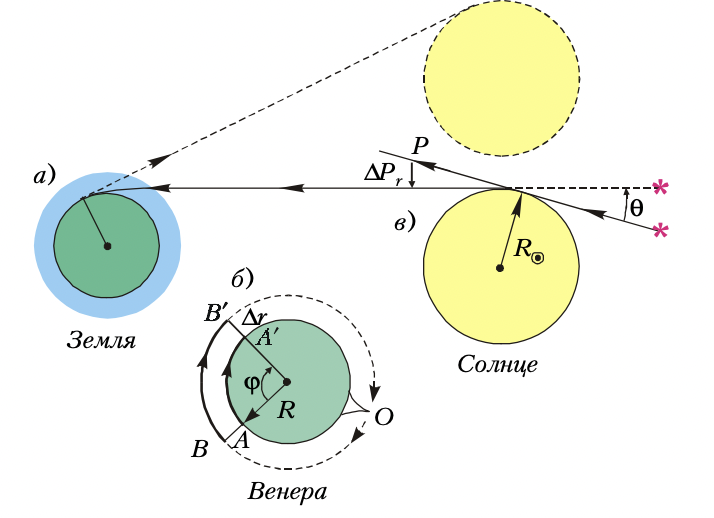
\includegraphics[width=0.8\linewidth]{1.png}
            
            \caption{Интересная картинка}
            
            \label{fig:mpr}
        
        \end{figure}
\end{document}
\overbrace{} 